%\documentclass[first,firstsupp,handout,compress,notes,navigation]{ETHclass} 
%\documentclass[first,firstsupp,handout,lastsupp]{ETHclass} 
\documentclass[first,firstsupp,lastsupp,handout,last,hyperref,table]{ETHclass} 
%\documentclass[first,firstsupp]{ETHclass}
\usepackage{etex}

\usepackage{adjustbox}
\usepackage{amsmath}
\usepackage{amssymb}
\usepackage{animate}
\usepackage{booktabs}
\usepackage{charter}
\usepackage{etoolbox}
\usepackage{ifthen}
\usepackage{longtable}
\usepackage{mathrsfs}
\usepackage{multicol}
\usepackage{pgf}
\usepackage{pgfplots}
\usepackage{pifont}
\usepackage{ragged2e}
\usepackage{standalone}
\usepackage[caption=false]{subfig}
\usepackage{tabularx}
\usepackage{tikz}
\usepackage{verbatim}
\usepackage{xcolor}
\usepackage{hyperref}



\setbeamertemplate{navigation symbols}{}
\usetikzlibrary{arrows,decorations.pathreplacing,positioning,shapes,shadows}

%\usepackage[style=numeric-comp]{biblatex}

%\usepackage{lipsum}

%\usetikzlibrary{fit}
\usetikzlibrary{arrows}
\usetikzlibrary{trees}

% Options for beamer:
%
% 9,10,11,12,13,14,17pt  Fontsizes
% 
% compress: navigation bar becomes smaller
% t       : place contents of frames on top (alternative: b,c)
% handout : handoutversion
% notes   : show notes
% notes=onlyslideswithnotes
%
%hyperref={bookmarksopen,bookmarksnumbered} : Needed for menues in
%                                             acrobat. Also need
%                                             pdftex as option or 
%                                             compile with
% pdflatex '\PassOptionsToPackage{pdftex,bookmarksopen,bookmarksnumbered}{hyperref} \input{file}'

%\usepackage{beamerseminar}
%\usepackage[accumulated]{beamerseminar}
                                % remove ``accumulated'' option
                                % for original behaviour
%\usepackage{beamerbasenotes}
%\setbeamertemplate{note page}[plain] 
%\setbeameroption{notes on second screen}

%\setbeamertemplate{note page}[plain] 
\setbeamertemplate{note page}{\ \\[.3cm]
\textbf{\color{blue}Notes:}\\%[0.1cm]
{\footnotesize %\tiny
\insertnote}}
%\setbeameroption{notes on second screen}


%\setbeamertemplate{navigation symbols}{} % suppresses all navigation symbols:
 \setbeamertemplate{navigation symbols}[horizontal] % Organizes the navigation symbols horizontally.
% \setbeamertemplate{navigation symbols}[vertical] % Organizes the navigation symbols vertically.
% \setbeamertemplate{navigation symbols}[only frame symbol] % Shows only the navigational symbol for navigating frames.

\setlayoutscale{0.5}
\setparametertextfont{\scriptsize}
\setlabelfont{\scriptsize}

% \useoutertheme[subsection=false]{miniframes}
% \usepackage{etoolbox}
% \makeatletter
% \patchcmd{\slideentry}{\advance\beamer@xpos by1\relax}{}{}{}
% \def\beamer@subsectionentry#1#2#3#4#5{\advance\beamer@xpos by1\relax}%
% \makeatother

% \makeatletter
%     \newenvironment{withoutheadline}{
%        \setbeamertemplate{headline}{%
% \vspace{15pt}
% }
%     }{}
% \makeatother

\makeatletter
    \newenvironment{withoutheadline}{
         \setbeamertemplate{headline}{%
\vspace{35pt}
}
        %\def\beamer@entrycode{\vspace*{-1.5\headheight}}
    }{}
\makeatother

\newcommand{\Cross}{$\mathbin{\tikz [x=1.4ex,y=1.4ex,line width=.2ex, red] \draw (0,0) -- (1,1) (0,1) -- (1,0);}$}%

\newcommand{\Checkmark}{$\color{green}\checkmark$}

\setbeamerfont{subsection in toc}{size=\tiny}

\makeatletter
\patchcmd{\beamer@sectionintoc}
  {\vfill}
  {\vskip1.5\itemsep}
  {}
  {}
\makeatother  

\setbeamertemplate{frametitle continuation}{}

\setbeamertemplate{bibliography entry title}{}
\setbeamertemplate{bibliography entry author}{}
\setbeamertemplate{bibliography entry location}{}
\setbeamertemplate{bibliography entry note}{}

\setbeamercolor*{bibliography entry title}{fg=black}
\setbeamercolor*{bibliography entry author}{fg=black}
\setbeamercolor*{bibliography entry location}{fg=black}
\setbeamercolor*{bibliography entry note}{fg=black}
% and kill the abominable icon
%\setbeamertemplate{bibliography item}{\color{forestgreen}$\blacktriangleright$}
\setbeamertemplate{bibliography item}{\insertbiblabel}
%\setbeamertemplate{bibliography item}{\theenumiv}

\newcommand{\highlightred}[1]{%
  \colorbox{red!50}{$\displaystyle#1$}}
  
\newcommand{\highlightyellow}[1]{%
  \colorbox{yellow!50}{$\displaystyle#1$}}
  
\newcommand{\highlightgreen}[1]{%
  \colorbox{green!50}{$\displaystyle#1$}}

\AtBeginSection[]{
  \begin{frame}
  \vfill
  \centering
  \begin{beamercolorbox}[sep=8pt,center,shadow=true,rounded=true]{title}
    \usebeamerfont{frametitle}\includegraphics[width=2ex]{freccia_trasparente_verde_foresta.png}\hspace{.5ex}~{\LARGE \textsc{\bfseries \insertsectionhead}}\par%
  \end{beamercolorbox}
  \vfill
  \end{frame}
}

\hyphenpenalty=5000
\tolerance=1000

\graphicspath{{figures/}}

\newenvironment{system}{\left\lbrace\begin{array}{@{}l@{}}}{\end{array}\right.}

\newenvironment{subsystem}{\left\lgroup\begin{array}{@{}l@{}}}{\end{array}\right.}

\defbeamertemplate*{title page}{customized}[1][]
{
\usebeamerfont{subtitle}
\usebeamercolor[fg]{subtitle}

\vspace{-1.75cm}

{\flushleft
 \usebeamerfont{title}{\inserttitle}\par
}
\vspace{-.25cm}
{\flushleft
 \usebeamerfont{subtitle}{\small \insertsubtitle} \par
}

%\vspace{-.5cm}

{\flushright
\setbeamercolor{author}{bg=white,fg=Red}
\usebeamerfont{author}{\footnotesize \insertauthor} \par}

\vspace{-.2cm}

{\flushright
\usebeamerfont{institute}{\tiny \insertinstitute}\par }

\vspace{.2cm}

{\centering
\usebeamerfont{date}{\scriptsize \insertdate} \par }

\vspace{0.2in}
}


\begin{document}
\setbeamertemplate{caption}{\raggedright\insertcaption\par}

\title[\textsc{FEM \& the Fiber-Matrix Interface Crack}]{\textsc{Finite Elements Solution of the Fiber-Matrix Interface Crack: Effects of Mesh Refinement and Domain Size}}
\author{ L. Di Stasio$^{1,2}$, Z. Ayadi$^{1}$, J. Varna$^{2}$}
%\institute{ Science et Ing\'enierie des Mat\'eriaux et M\'etallurgie (SI2M), Institut Jean Lamour, Nancy, France\\Department of Engineering Sciences and Mathematics, Division of Materials Science, Lule\aa\ University of Technology, Lule\aa, Sweden}
\institute{$^{1}$EEIGM, Universit\'e de Lorraine, Nancy, France\\$^{2}$Division of Materials Science, Lule\aa\ University of Technology, Lule\aa, Sweden}
\date{DocMASE Summer School, Sarrebr\"ucken (DE) - Nancy (FR), September 11 - 15, 2017}

\begin{frame}[plain]
    \titlepage
\end{frame}

\begin{withoutheadline}
\begin{frame}
\frametitle{Outline}
\justifying
\vspace*{-0.5cm}
% \tableofcontents[hidesubsections]
% \begin{multicols}{2}
% \tableofcontents[hidesubsections]
% \end{multicols}
% \begin{columns}[t]
%         \begin{column}{.5\textwidth}
%             \tableofcontents[sections={1-2}]
%         \end{column}
%         \begin{column}{.5\textwidth}
%             \tableofcontents[sections={3-6}]
%         \end{column}
%     \end{columns}
% \end{frame}
\tableofcontents[hidesubsections]
\end{frame}
\end{withoutheadline}

%\note{}

%\begin{frame}
%\pagediagram
%\end{frame}
%% \note{}

\section[The Fiber-Matrix Interface Problem in FRPC]{The Fiber-Matrix Interface Problem in Fiber Reinforced Polymer Laminates}

\subsection{The Fiber-Matrix Interface Problem}

\subsection{Intralaminar Transverse Cracking}

\begin{frame}
\frametitle{Intralaminar Transverse Cracking}
\vspace{-0.75cm}
\centering
\captionsetup[subfigure]{labelfont=footnotesize}
\begin{figure}[!h]
\centering
\subfloat[\scriptsize By Dr. R. Olsson, Swerea, SE.\label{fig:all-cracks}]{\includegraphics[width=0.46\textwidth]{all-cracks.png}}\quad
\subfloat[\scriptsize By Prof. Dr. E. K. Gamstedt, KTH, SE.\label{fig:transverse-cracks}]{\includegraphics[width=0.5\textwidth]{intralaminar-cracks.png}}
 \caption{A visual definition of intralaminar transverse cracking.}
  \label{fig:intralaminar-cracks}
\end{figure}
\end{frame}

\begin{frame}
\frametitle{Characterization of the Fracture Process}
\vspace{-0.5cm}
\centering

\end{frame}

\begin{frame}
\frametitle{The Fiber-Matrix Interface Crack}
\vspace{-0.5cm}
\centering

\end{frame}

\section{Objectives \& Approach}

\begin{frame}
\frametitle{Objectives \& Approach}
\vspace{-0.25cm}
\centering
\scriptsize
\begin{alertblock}{\small \bf{Objectives}}
\begin{itemize}
    \item Investigate the influence of volume fraction, thin ply thickness and bounding plies' thicknesses on crack initiation 
    \item To infere a relationship like
	\begin{equation*}
		G_{*c}=G_{*c}\left(\theta_{debond},\Delta\theta_{debond}, E_{\left(\cdot\cdot\right)}, \nu_{\left(\cdot\cdot\right)}, G_{\left(\right)},VF_{f}, t_{ply}, \frac{t_{ply}}{t_{bounding\ plies}}\right)
	\end{equation*}
\end{itemize}
\end{alertblock}
\begin{alertblock}{\small \bf{Approach}}
\begin{itemize}
    \item Design and categorization of different Representative Volume Elements (RVEs)
    \item Automated generation of RVEs geometry and FEM model
    \item Finite Element Simulation (in Abaqus)
\end{itemize}
\end{alertblock}
\end{frame}

\section{Micromechanical modeling}

\subsection[RVEs' Design]{Representative Volume Elements' (RVEs) Design}

\begin{frame}
\frametitle{From macro to micro}
\vspace{-1cm}
\centering
\begin{figure}
\centering
\includegraphics[height=0.85\textheight]{laminate-section.pdf}
%\caption{}
\label{fig:spread-tow-schematic}
\end{figure}
\end{frame}

\begin{frame}
\frametitle{Representative Volume Elements (RVEs)}
\vspace{-0.75cm}
\centering
\begin{figure}
\centering
\includegraphics[height=0.8\textheight]{periodicRVE_cc.pdf}
%\caption{\scriptsize Visualization of reference RVE inside a periodic square-array structure.}
\label{fig:periodicRVE}
\end{figure}
\end{frame}

\subsection[Mesh Design]{Mesh Design and Generation}

\begin{frame}
\frametitle{\vspace*{0.25cm}\small Mesh Design and Generation}
\vspace{-0.5cm}
\centering
\tiny
\begin{alertblock}{\scriptsize \bf{Why a good mesh is fundamental}}
\begin{enumerate}
\item Geometric discretization has a strong effect on non-linear FEM simulations 
\item Damage is a process that implies changes in geometry, i.e. generation of surfaces and domain splitting
\item Fracture mechanics quantities depends on the local mesh topology and refinement 
\end{enumerate}
\end{alertblock}
\begin{alertblock}{\scriptsize \bf{4-step procedure for mesh generation}}
\begin{enumerate}
\item The boundary is generated patching analytical parameterizations
\item The boundary is split into a set of 4 corners ($c_{i}$) and 4 edges ($e_{i}$)
\item Interior nodes are created applying transfinite interpolation using multi-dimensional linear Lagrangian interpolants

\begin{equation*}
P_{1}(x,p_{j})=\sum_{j=1}^{n}p_{j}\prod_{k=1\ k\neq j}^{n}\frac{x-x_{k}}{x_{j}-x_{k}}\quad P_{2}(x,y,p_{j},q_{j})=P_{1}(x,p_{j})\otimes P_{1}(y,q_{j})
\end{equation*}

\begin{equation*}
r(\xi,\eta)=P_{1}(\xi,e_{2},e_{4})+P_{1}(\eta,e_{1},e_{3})- P_{2}(\xi,\eta,c_{1},c_{2},c_{3},c_{4})
\end{equation*}

\item The mesh is smoothed applying elliptic mesh generation

\begin{equation*}
g^{11}\underline{r}_{,\xi\xi}+2g^{12}\underline{r}_{,\xi\eta}+g^{22}\underline{r}_{,\eta\eta}=0
\end{equation*}

\end{enumerate}
\end{alertblock}
\end{frame}


\begin{frame}
\frametitle{Angular discretization}
\vspace{-0.7cm}
\centering
\captionsetup[figure]{font=scriptsize,labelfont=scriptsize}
\begin{figure}[!h]
\centering
\includegraphics[height=0.7\textheight]{mesh-disc-at-interface.pdf}
  \caption{Angular discretization at fiber/matrix interface: $\delta=\frac{360^{\circ}}{4N_{\alpha}}$.}
  \label{fig:angu-discr-def}
\end{figure}
\end{frame}

\subsection[FEM Model]{Finite Element Model in Abaqus}

\subsection[$G_{c}$ Numerical Evaluation]{Numerical Evaluation of Energy Release Rate}

\begin{frame}
\frametitle{Virtual Crack Closure Technique (VCCT)}
\vspace{-1.5cm}
\centering
\begin{figure}[!h]
\centering
\includegraphics[height=0.6\textheight]{VCCT.pdf}
 % \caption{Angular discretization at fiber/matrix interface.}
  \label{fig:vcct}
\end{figure}
\begin{equation*}
G_{I}=\frac{Z_{C}\Delta w_{C}}{2B\Delta a}\quad G_{II}=\frac{X_{C}\Delta u_{C}}{2B\Delta a}\quad\Longleftrightarrow\quad\text{In-house routine and Abaqus built-in *DEBOND function}
\end{equation*}
\end{frame}

\begin{frame}
\frametitle{J-integral evaluation}
\vspace{-0.75cm}
\centering
\begin{figure}[!h]
\centering
\includegraphics[height=0.6\textheight]{J-integral.pdf}
 % \caption{Angular discretization at fiber/matrix interface.}
  \label{fig:jintegral}
\end{figure}
\scriptsize
\begin{equation*}
J_{i}=\lim_{\varepsilon\to 0}\int_{\Gamma_{\varepsilon}}\left(W\left(\Gamma\right)n_{i}-n_{j}\sigma_{jk}\frac{\partial u_{k}\left(\Gamma,x_{i}\right)}{\partial x_{i}}\right)d\Gamma\Longleftrightarrow\text{*CONTOUR INTEGRAL in Abaqus}
\end{equation*}
\end{frame}

\section[Results]{Preliminary Results \& Perspectives}

\subsection{$\sigma_{0}$ and $G_{0}$}

\begin{frame}
\frametitle{\small $\sigma_{0}$ for $Vf_{f}=0.001$, $\frac{L}{R_{f}}\sim28$ and $\delta=0.4^{\circ}$}
\vspace{-0.5cm}
\centering
\captionsetup[figure]{font=scriptsize,labelfont=scriptsize}
\begin{figure}[!h]
\centering
\includegraphics[height=0.7\textheight]{2017-06-23_AbqRunSummary_SingleFiberEqRfSmallFiniteStrain_sigma-inf_Summary.pdf}
  \caption{\scriptsize In red small strain FEM, in green finite strain FEM, in black $\sigma_{0}=\frac{E}{1-\nu^{2}}\varepsilon$.}
  \label{fig:res1}
\end{figure}
\end{frame}

\begin{frame}
\frametitle{\small $G_{0}$ for $Vf_{f}=0.001$, $\frac{L}{R_{f}}\sim28$ and $\delta=0.4^{\circ}$}
\vspace{-0.5cm}
\centering
\captionsetup[figure]{font=scriptsize,labelfont=scriptsize}
\begin{figure}[!h]
\centering
\includegraphics[height=0.7\textheight]{2017-06-23_AbqRunSummary_SingleFiberEqRfSmallFiniteStrain_G0_Summary.pdf}
  \caption{\scriptsize In red small strain FEM, in green finite strain FEM, in black $G_{0}$ calculated assuming $\sigma_{0}=\frac{E}{1-\nu^{2}}\varepsilon$.}
  \label{fig:res1}
\end{figure}
\end{frame}

\begin{frame}
\frametitle{\small $\sigma_{0}$ for $Vf_{f}=0.000079$, $\frac{L}{R_{f}}\sim100$ and $\delta=0.4^{\circ}$}
\vspace{-0.5cm}
\centering
\captionsetup[figure]{font=scriptsize,labelfont=scriptsize}
\begin{figure}[!h]
\centering
\includegraphics[height=0.7\textheight]{2017-06-16_AbqRunSummary_SingleFiberEqRfSmallStrain-D0-4_sigma-inf_Summary.pdf}
  \caption{\scriptsize In red small strain FEM, in black $\sigma_{0}=\frac{E}{1-\nu^{2}}\varepsilon$.}
  \label{fig:res1}
\end{figure}
\end{frame}

\begin{frame}
\frametitle{\small $G_{0}$ for $Vf_{f}=0.000079$, $\frac{L}{R_{f}}\sim100$ and $\delta=0.4^{\circ}$}
\vspace{-0.5cm}
\centering
\captionsetup[figure]{font=scriptsize,labelfont=scriptsize}
\begin{figure}[!h]
\centering
\includegraphics[height=0.7\textheight]{2017-06-16_AbqRunSummary_SingleFiberEqRfSmallStrain-D0-4_G0_Summary.pdf}
  \caption{\scriptsize In red small strain FEM, in black $G_{0}$ calculated assuming $\sigma_{0}=\frac{E}{1-\nu^{2}}\varepsilon$.}
  \label{fig:res1}
\end{figure}
\end{frame}

%\begin{frame}
%\frametitle{\small Conclusions}
%\vspace{-0.5cm}
%\centering
%\begin{itemize}[label=\ding{212}]
%\item $\sigma_{0}$ and $G_{0}$ depend on $\Delta\theta$ for finite sizes of the RVE
%\item As the RVE size $\rightarrow\infty$, i.e. $\frac{L}{R_{f}}\rightarrow \infty$ ($\sim 100$), $\sigma_{0}$ and $G_{0}$ tend to the theoretical undamaged value given by $\sigma_{0}=\frac{E_{m}}{1-\nu_{m}^{2}}\varepsilon_{0}$
%\item $\sigma_{0}$ and $G_{0}$ might be taken as a good measure of "infinetess" for strain-/displacement-controlled simulations
%\item By selecting $\Delta\theta=10^{\circ}$ and running a parametric study with a comparatevely coarse mesh the minimum ratio  $\frac{L}{R_{f}}$ or equivalently maximum $Vf_{f}$ volume to have an infinite RVE could be found
%\end{itemize}
%\end{frame}

\subsection{Finite strain and small strain formulations}

\begin{frame}
\frametitle{\small $\frac{G_{\left(\cdot\cdot\right)}}{G_{0}}$ for $V_{f}=0.001$, $\frac{L}{R_{f}}\sim28$ and $\delta=0.4^{\circ}$}
\vspace{-0.5cm}
\centering
\captionsetup[figure]{font=scriptsize,labelfont=scriptsize}
\begin{figure}[!h]
\centering
\includegraphics[height=0.7\textheight]{2017-06-23_AbqRunSummary_SingleFiberEqRfSmallFiniteStrain_M-VCCT_Summary.pdf}
  \caption{\scriptsize In red small strain FEM, in green finite strain FEM, in black BEM results.}
  \label{fig:res1}
\end{figure}
\end{frame}

\begin{frame}
\frametitle{\small $\frac{G_{\left(\cdot\cdot\right)}}{G_{0}}$ for $V_{f}=0.001$, $\frac{L}{R_{f}}\sim28$ and $\delta=0.4^{\circ}$, small strain formulation}
\vspace{-0.5cm}
\centering
\captionsetup[figure]{font=scriptsize,labelfont=scriptsize}
\begin{figure}[!h]
\centering
\includegraphics[height=0.7\textheight]{2017-06-23_AbqRunSummary_SingleFiberEqRfSmallStrain_J-INT_Summary.pdf}
  \caption{\scriptsize Fading from blue to red J-Integrals evaluated at contours at increasing distance from the crack tip, in black BEM results.}
  \label{fig:res1}
\end{figure}
\end{frame}

\begin{frame}
\frametitle{\small $\frac{G_{\left(\cdot\cdot\right)}}{G_{0}}$ for $V_{f}=0.001$, $\frac{L}{R_{f}}\sim28$ and $\delta=0.4^{\circ}$, small strain formulation}
\vspace{-0.5cm}
\centering
\captionsetup[figure]{font=scriptsize,labelfont=scriptsize}
\begin{figure}[!h]
\centering
\includegraphics[height=0.7\textheight]{2017-06-23_AbqRunSummary_SingleFiberEqRfSmallStrain_VCCT-JINT_Summary.pdf}
  \caption{\scriptsize Fading from blue to red J-Integrals evaluated at contours at increasing distance from the crack tip, in green evaluation with in-house VCCT routine, in black BEM results.}
  \label{fig:res1}
\end{figure}
\end{frame}

\begin{frame}
\frametitle{\small $\frac{G_{\left(\cdot\cdot\right)}}{G_{0}}$ for $V_{f}=0.001$, $\frac{L}{R_{f}}\sim28$ and $\delta=0.4^{\circ}$, finite strain formulation}
\vspace{-0.5cm}
\centering
\captionsetup[figure]{font=scriptsize,labelfont=scriptsize}
\begin{figure}[!h]
\centering
\includegraphics[height=0.7\textheight]{2017-06-23_AbqRunSummary_SingleFiberEqRfFiniteStrain_J-INT_Summary.pdf}
  \caption{\scriptsize Fading from blue to red J-Integrals evaluated at contours at increasing distance from the crack tip, in black BEM results.}
  \label{fig:res1}
\end{figure}
\end{frame}

\begin{frame}
\frametitle{\small $\frac{G_{\left(\cdot\cdot\right)}}{G_{0}}$ for $V_{f}=0.001$, $\frac{L}{R_{f}}\sim28$ and $\delta=0.4^{\circ}$, finite strain formulation}
\vspace{-0.5cm}
\centering
\captionsetup[figure]{font=scriptsize,labelfont=scriptsize}
\begin{figure}[!h]
\centering
\includegraphics[height=0.7\textheight]{2017-06-23_AbqRunSummary_SingleFiberEqRfFiniteStrain_VCCT-JINT_Summary.pdf}
  \caption{\scriptsize Fading from blue to red J-Integrals evaluated at contours at increasing distance from the crack tip, in green evaluation with in-house VCCT routine, in black BEM results.}
  \label{fig:res1}
\end{figure}
\end{frame}

%\begin{frame}
%\frametitle{\small Conclusions}
%\vspace{-0.5cm}
%\centering
%\begin{itemize}[label=\ding{212}]
%\item For both small and finite strain formulations, J-integrals are already in good agreement with $\frac{G_{TOT}}{G_{0}}$ from BEM, i.e. no sizeable finite size effect already at $\frac{L}{R_{f}}\sim 28$
%\item For both small and finite strain formulations, J-integrals correct measure the peak value of $\frac{G_{TOT}}{G_{0}}$ at $60^{\circ}$
%\item J-Integrals in small strain slightly overestimate the BEM result
%\item J-integrals in small strain shows poor convergence in the range $50^{\circ}-80^{\circ}$
%\item J-Integrals in finite strain slightly underestimate the BEM result
%\item J-integrals in finite strain shows very good convergence in all the range $10^{\circ}-150^{\circ}$
%\end{itemize}
%\end{frame}

%\begin{frame}
%\frametitle{\small Conclusions}
%\vspace{-0.5cm}
%\centering
%\begin{itemize}[label=\ding{212}]
%\item $\frac{G_{TOT}}{G_{0}}$ is correctly calculated by the VCCT in small strain, in good agreement with BEM results
%\item $\frac{G_{TOT}}{G_{0}}$ is wrongly calculated by the VCCT in finite strain, with a peak at $65^{\circ}-70^{\circ}$
%\item Small strain VCCT shows better results than finite strain VCCT
%\item Mode ratio is still not correct, i.e. probably finite size effect
%\end{itemize}
%\end{frame}

%\begin{frame}
%\frametitle{\small Observations \& Questions}
%\vspace{-0.45cm}
%\centering
%\begin{itemize}[label=\ding{212}]
%\item J-Integral is a far-field technique, using stresses, strain and displacements far from the crack tip; convergence is in fact far from crack tip (at least 10 contours, i.e. 10 ring of elements)
%\item VCCT is a local technique, using forces and displacements at the crack tip
%\item The difference between small and finite strain results rests mainly in the displacements
%\item Previously, we observed that changing the formulation of the bonded interface, all other parameters equal, the result doesn't change
%\item All the convergence problem reduces to the correct evaluation of displacements of debonded surfaces close to the crack tip
%\item Displacements of debonded surfaces close to the crack tip are influenced by RVE size
%\end{itemize}
%\end{frame}

%\begin{frame}
%\frametitle{\small Observations \& Questions}
%\vspace{-0.25cm}
%\centering
%\begin{itemize}[label=\ding{212}]
%\item Small strain shows (correctly) better results than finite strain formulation with respect to infinite reference values
%\item However, Abaqus documentation suggests that, if contact between surfaces is present in the model, finite strain formulation (nonlinear geometry) should be used
%\item For finite sizes of RVE, which formulation should be chosen?
%\end{itemize}
%\end{frame}

%\subsection{Elements's aspect ratio}
%
%\begin{frame}
%\frametitle{\small $\frac{G_{\left(\cdot\cdot\right)}}{G_{0}}$ for  $Vf_{f}=0.000079$, $\frac{L}{R_{f}}\sim100$ and $\delta=1.0^{\circ}$, small strain formulation}
%\vspace{-0.5cm}
%\centering
%\captionsetup[figure]{font=scriptsize,labelfont=scriptsize}
%\begin{figure}[!h]
%\centering
%\includegraphics[height=0.7\textheight]{2017-06-16_AbqRunSummary_SingleFiberEqRfSmallStrain-D1-0_VCCT-JINT_Summary.pdf}
%  \caption{\scriptsize Fading from blue to red J-Integrals evaluated at contours at increasing distance from the crack tip, in green evaluation with in-house VCCT routine, in black BEM results.}
%  \label{fig:res1}
%\end{figure}
%\end{frame}
%
%\begin{frame}
%\frametitle{\small $\frac{G_{\left(\cdot\cdot\right)}}{G_{0}}$ for  $Vf_{f}=0.000079$, $\frac{L}{R_{f}}\sim100$ and $\delta=0.4^{\circ}$, small strain formulation}
%\vspace{-0.5cm}
%\centering
%\captionsetup[figure]{font=scriptsize,labelfont=scriptsize}
%\begin{figure}[!h]
%\centering
%\includegraphics[height=0.7\textheight]{2017-06-16_AbqRunSummary_SingleFiberEqRfSmallStrain-D0-4_VCCT-JINT_Summary.pdf}
%  \caption{\scriptsize Fading from blue to red J-Integrals evaluated at contours at increasing distance from the crack tip, in green evaluation with in-house VCCT routine, in black BEM results.}
%  \label{fig:res1}
%\end{figure}
%\end{frame}

%\begin{frame}
%\frametitle{\small Conclusions}
%\vspace{-0.5cm}
%\centering
%\begin{itemize}[label=\ding{212}]
%\item Elements' aspect ratio (maximum side length/minimum side length) was very high in the exterior part of the matrix in this set of simulations
%\item Spurious stresses adn deformations were created at $45^{\circ},135^{\circ},225^{\circ},315^{\circ}$
%\item Results are badly affected by this in the range  $40^{\circ} - 70^{\circ}$ with a marked oscillation between $40^{\circ} - 50^{\circ}$
%\item Elements' aspect ratio in the matrix is more important than the elements' size at the fiber/matrix interface
%\item Program has already been changed to receive aspect ratios as input instead of number of elements
%\item Results from previous sections were calculated with meshes with controlled aspect ratios
%\end{itemize}
%\end{frame}



%\begin{frame}
%\frametitle{$\sigma_{xx}$ along radial sections}
%\vspace{-0.35cm}
%\centering
%\captionsetup[subfigure]{font=scriptsize,labelfont=scriptsize}
%\begin{figure}[!h]
%\centering
%\includegraphics[height=0.7\textheight]{AllRadialSections-S11.pdf}
% \caption{$\Delta\theta=5^{\circ},\delta=0.4^{\circ},VF_{f}=0.001,\frac{l}{R_{f}}\approx28$}
%  \label{fig:allradialS11}
%\end{figure}
%\end{frame}
%
%\begin{frame}
%\frametitle{$\sigma_{zz}$ along radial sections}
%\vspace{-0.35cm}
%\centering
%\captionsetup[subfigure]{font=scriptsize,labelfont=scriptsize}
%\begin{figure}[!h]
%\centering
%\includegraphics[height=0.7\textheight]{AllRadialSections-S22.pdf}
% \caption{$\Delta\theta=5^{\circ},\delta=0.4^{\circ},VF_{f}=0.001,\frac{l}{R_{f}}\approx28$}
%  \label{fig:allradialS22}
%\end{figure}
%\end{frame}
%
%\begin{frame}
%\frametitle{$\tau_{xz}$ along radial sections}
%\vspace{-0.35cm}
%\centering
%\captionsetup[subfigure]{font=scriptsize,labelfont=scriptsize}
%\begin{figure}[!h]
%\centering
%\includegraphics[height=0.7\textheight]{AllRadialSections-S12.pdf}
% \caption{$\Delta\theta=5^{\circ},\delta=0.4^{\circ},VF_{f}=0.001,\frac{l}{R_{f}}\approx28$}
%  \label{fig:allradialS12}
%\end{figure}
%\end{frame}

\section[Conclusions]{Conclusions \& Outlook}

\begin{frame}
\frametitle{\vspace*{0.5cm} Conclusions \& Outlook}
\vspace{-0.75cm}
\centering
\scriptsize
\begin{alertblock}{\footnotesize \bf{Conclusions}}
\begin{itemize}
   	\item 2D micromechanical models have been developed to investigate crack initiation in thin ply laminates
	\item A numerical procedure has been devised and implemented to automatize the creation of FEM models
	\item Analyses for $VF_{f}\to 0$ (matrix dominated RVE) conducted to validate the model with respect to previous literature
\end{itemize}
\end{alertblock}
\begin{alertblock}{\footnotesize \bf{Outlook}}
\begin{itemize}
	\item Investigate the dependence on $VF_{f}$, $t_{ply}$, $\frac{t_{ply}}{t_{bounding\ plies}}$ and different material systems\\[9pt]
	\item Study numerical performances with respect to model's parameters\\[9pt]
	\item Repeat for different RVEs and compare
\end{itemize}
\end{alertblock}
\end{frame}

\section{Appendices \& References}

\subsection{Appendices}

%\begin{frame}[label=]
%\frametitle{}
%\end{frame}

\begin{frame}
\frametitle{Spread Tow Technology: Implications}
\vspace{-0.75cm}
\centering
\begin{itemize}
	\item Strong reduction in ply's thickness and weight
	\item Reduction in laminate's thickness and weight
	\item Higher fiber volume fraction and more homogeneous fiber distribution
	\item Ply thickness to fiber diameter ratio decreases of at least 1 order of magnitude, from $>100$ to $\leq10$
	\item Increased load at damage onset and increased ultimate strength, in particular for transverse cracking
\end{itemize}
\end{frame}

\begin{frame}
\frametitle{RVEs: Variations on a Theme}
\vspace{-0.75cm}
\centering
\begin{figure}[!h]
\centering
\subfloat{\includegraphics[height=0.4\textheight]{SingleRVEs.pdf}}\quad
\subfloat{\includegraphics[height=0.4\textheight]{boundedRVE_cc.pdf}}\quad
\subfloat{\includegraphics[height=0.4\textheight]{periodicRVE_cc.pdf}}
  %\caption{Single RVE model.}
  \label{fig:RVEs-variations}
\end{figure}
\end{frame}

\begin{frame}
\frametitle{RVEs: First Variation on a Theme}
\vspace{-0.25cm}
\centering
\begin{figure}
\centering
\includegraphics[height=0.7\textheight]{LEFM2DsRVEsFsDdepverdispBCULappAxialDispLR.pdf}
\caption{\scriptsize Isolated RVE with zero vertical displacement BC.}
\label{fig:singleRVE-rigid}
\end{figure}
\end{frame}

\begin{frame}
\frametitle{RVEs: Second Variation on a Theme}
\vspace{-0.25cm}
\centering
\begin{figure}
\centering
\includegraphics[height=0.7\textheight]{LEFM2DsRVEsFsDhomoBCULappAxialDispLR.pdf}
\caption{\scriptsize Isolated RVE with homogeneous displacement BC.}
\label{fig:singleRVE-homo}
\end{figure}
\end{frame}

\begin{frame}
\frametitle{RVEs: Third Variation on a Theme}
\vspace{-0.25cm}
\centering
\begin{figure}
\centering
\includegraphics[height=0.7\textheight]{boundedRVE_cc.pdf}
\caption{\scriptsize Bounded RVE.}
\label{fig:boundedRVE}
\end{figure}
\end{frame}

\begin{frame}
\frametitle{Topological transformation}
\vspace{-1cm}
\centering
\captionsetup[subfigure]{font=scriptsize,labelfont=scriptsize}
\begin{figure}[!h]
\centering
\subfloat[]{\includegraphics[height=0.4\textheight]{mesh_regions.pdf}}\qquad
\subfloat[]{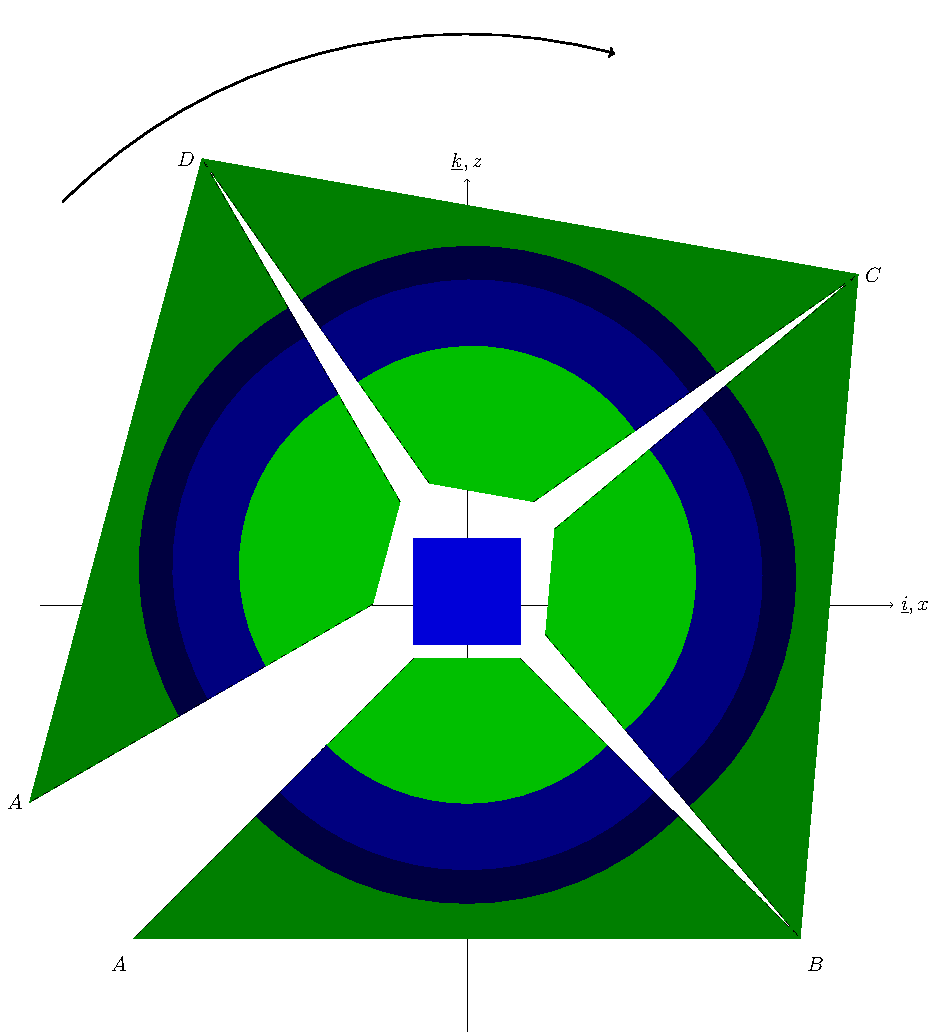
\includegraphics[height=0.4\textheight]{opening1.pdf}}\\
\subfloat[]{\includegraphics[height=0.3\textheight]{opening2.pdf}}\qquad
\subfloat[]{\includegraphics[width=0.6\textwidth]{opening3.pdf}}
  %\caption{Single RVE model.}
  \label{fig:topological-geom-transf}
\end{figure}
\end{frame}

\begin{frame}
\frametitle{Mesh parameters}
\vspace{-0.7cm}
\centering
\captionsetup[subfigure]{font=scriptsize,labelfont=scriptsize}
\begin{figure}[!h]
\centering
\subfloat{\includegraphics[height=0.75\textheight]{mesh_parameters_single.pdf}}\qquad
\subfloat{\includegraphics[height=0.75\textheight]{mesh_parameters_bounded.pdf}}
  %\caption{Single RVE model.}
  \label{fig:mesh-params}
\end{figure}
\end{frame}

\begin{frame}
\frametitle{Finite Element Model in Abaqus}
\vspace{-0.7cm}
\centering
\captionsetup[figure]{font=scriptsize,labelfont=scriptsize}
\begin{table}[h!]
\scriptsize
  \centering
  %\caption{Analysis methods summary.}
    \begin{tabularx}{\textwidth}{X}
    \toprule
    \midrule    
    \textbf{Method}\\
    ABAQUS/STD static analysis + VCCT + J-integral.\\
    \midrule
    \textbf{Type}\\
    Static, i.e. no inertial effects. Relaxation until equilibrium.\\
    \midrule
    \textbf{Elements}\\
    CPE4/CPE8\\
    \midrule
    \textbf{Interface}\\
    Tied surface constraint \& contact mechanics\\
    \midrule
   \textbf{Input variables}\\
    $R_{f}$, $V_{f}$, material properties, interface properties.\\
    \midrule
    \textbf{Control variables}\\
    $\theta$, $\Delta\theta$, $\bar{\varepsilon}_{x}$.\\
    \midrule
 \textbf{Output variables} \\
  Stress field, crack tip stress, stress intensity factors, energy release rates, $a$.\\
  \midrule
    \bottomrule
    \end{tabularx}%
  \label{tab:analysis_tab}%
\end{table}
\end{frame}

\begin{frame}
\frametitle{\small Evaluation of $G_{0}$}
\vspace{-0.7cm}
\footnotesize
\centering
\captionsetup[figure]{font=scriptsize,labelfont=scriptsize}
\begin{equation}
G_{0}=\pi R_{f}\sigma^{2}_{0}\frac{1+k_{m}}{8G_{m}}
\end{equation}
\begin{equation}
k_{m}=3-4\nu_{m}
\end{equation}
\begin{equation}
\sigma_{0}^{undamaged}=\frac{E_{m}}{1-\nu^{2}_{m}}\varepsilon_{xx}
\end{equation}%
\end{frame}


%\section{References}

%\begin{frame}[t,label=references,allowframebreaks]
%       \frametitle{References}
%	\begin{itemize}
%%	\item Loading rate effects on delamination:\\[10pt] \textit{Loading\_rate\_effects\_on\_CFRP.bib}\\[30pt]
%	\item Body-fitted grids for FSI modeling with LBM:\\[10pt] %\textit{Fluid\_structure\_interaction\_on\_deformable\_surfaces.bib}
%	\end{itemize}
%        \bibliographystyle{amsalpha}
%        {\footnotesize
%          \bibliography{PSI_talk.bib}
%        }
        %\bibliography{/auto.mounter/home/lucadistasio/Documents/ETH/Research_material/References/fsi_references_kbib.bib}
%\end{frame}

\subsection{References}

\begin{frame}[allowframebreaks]
  \frametitle{References}
    
  \begin{thebibliography}{10}
    
%  \beamertemplatebookbibitems
%  % Start with overview books.
%
%  \bibitem{Author1990}
%    A.~Author.
%    \newblock {\em Handbook of Everything}.
%    \newblock Some Press, 1990.
 
    
  \beamertemplatearticlebibitems
  % Followed by interesting articles. Keep the list short. 

\bibitem{DonaldL.Flaggs1982}
Donald L. Flaggs, Murat H. Kural;
\newblock {\em Experimental Determination of the In Situ Transverse Lamina Strength in Graphite/Epoxy Laminates.}
\newblock Journal of Composite Materials, vol. 16, n. 2, 1982.

\bibitem{Parvizi1978}
Parvizi A., Bailey J.E;
\newblock {\em On multiple transverse cracking in glass fibre epoxy cross-ply laminates.}
\newblock Journal of Materials Science, 1978; 13:2131-2136.

\bibitem{herraez2015}
Miguel Herr\'aez, Diego Mora, Fernando Naya, Claudio S. Lopes, Carlos Gonz\'alez, Javier LLorca;
\newblock {\em Transverse cracking of cross-ply laminates: A computational micromechanics perspective.}
\newblock Composites Science and Technology, 2015; 110:196-204.

\bibitem{Canal2012}
Luis Pablo Canal, Carlos Gonz\'alez, Javier Segurado, Javier LLorca;
\newblock {\em Intraply fracture of fiber-reinforced composites: Microscopic mechanisms and modeling.}
\newblock Composites Science and Technology, 2012; 72(11):1223-1232.

\bibitem{StephenW.Tsai2005}
Stephen W. Tsai;
\newblock {\em Thin ply composites.}
\newblock JEC Magazine 18, 2005.


\bibitem{ZnedekP.Bazant2002}
Znedek P. Bazant;
\newblock {\em Size Effect Theory and its Application to Fracture of Fiber Composites and Sandwich Plates.} 
\newblock in Continuum Damage Mechanics of Materials and Structures, eds. O. Allix and F. Hild, 2002.


\bibitem{RobinAmacherWayneSmithClemensDransfeldJohnBotsis2014}
Robin Amacher, Wayne Smith, Clemens Dransfeld, John Botsis, Jo\"el Cugnoni;
\newblock {\em Thin Ply: from Size-Effect Characterization to Real Life Design}
\newblock CAMX 2014, 2014

\bibitem{RalfCuntze}
Ralf Cuntze;
\newblock {\em The  World-Wide-Failure-Exercises -I  and - II for UD-materials.}


\bibitem{Pinho}
Pinho, S. T. and Pimenta, S.;
\newblock {\em Size Effects on the Strength and Toughness of Fibre-Reinforced Composites.}

\bibitem{PedroP.CamanhoCarlosG.DavilaSilvestreT.PinhoLorenzoIannucci2006}
Pedro P. Camanho, Carlos G. D\'avila, Silvestre T. Pinho, Lorenzo Iannucci, Paul Robinson;
\newblock {\em Prediction of in situ strengths and matrix cracking in composites under transverse tension and in-plane shear.}
\newblock Composites Part A: Applied Science and Manufacturing, vol. 37, n. 2, 2006.

\bibitem{P.P.CamanhoP.Maimi2007}
P.P. Camanho, P. Maim\'i, C.G. D\'avila;
\newblock {\em Prediction of size effects in notched laminates using continuum damage mechanics.}
\newblock Composites Science and Technology, vol. 67, n. 13, 2007.

\bibitem{Nairn1992}
J. A. Nairn;
\newblock {\em The Initiation and Growth of Delaminations Induced by Matrix Microcracks in Laminated Composites.}
\newblock International Journal of Fracture, vol. 57, 1992.

\bibitem{JoelCugnoniRobinAmacher2013}
Joel Cugnoni , Robin Amacher, John Botsis;
\newblock {\em Thin ply technology advantages. An overview of the TPT-TECA project.}
\newblock 2014.

\bibitem{DonaldL.Flaggs1982}
Donald L. Flaggs, Murat H. Kural;
\newblock {\em Experimental Determination of the In Situ Transverse Lamina Strength in Graphite/Epoxy Laminates.}
\newblock Journal of Composite Materials, vol. 16, n. 2, 1982.

  \end{thebibliography}
\end{frame}

\begin{frame}[plain]
\frametitle{}
\end{frame}

\end{document}

